 \section{Overview and common stuff}

There are several things you should know when you read
the kernel program codes.

\subsection{Coding rule of \NICAM}

\NICAM is written with Fortran90/95 standards, and uses \src{module} to
modularize the program.
%
Module name begins with \src{mod_}, such as \src{mod_adm}.
%
Almost all source file defines only one module and have the same name
with the module, such as \file{mod_adm.f90}
%
Several modules are used to define public parameters, variables, and
subroutines, called ``public object''.
%
Name of such objects are prefixed its module name.
%
For example, \src{ADM_gall} is defined in module \src{mod_adm} that is
defined in \file{mod_adm.f90} in original \NICAM source.
%
Among the public objects, variables and parameters related to the
problem size are moved and defined in \file{problem_size.inc}, that is
included in \file{mod_misc.f90}

\subsection{Data array for regular region}

\autoref{f:data_store_regular} shows the schematic figure of data layout
in a regular region.
%
The grid points managed in the region are black circles, and white and
blue circles are so called ``halo points'', these are used only for the
reference and their values are provided from the neighboring regions by
the MPI communication or memory copy.
%
If the west-most vertex of the region is the vertex of the original
icosahedron, called singular points, two blue points have the same
value.
%
As you can see in \autoref{f:data_store_regular}, all grid points can be
specified by two index $i$ and $j$, in the direction of southward and
northword, respectively.
%
For the computational efficiency, especially for vectorizing or using
SIMD, the $i$ and $j$ dimension are merged, so usual variables are
defined in a form shown in \autoref{t:data_array_regular}.
%
The first dimensions corresponds to the horizontal index, the second is
vertical index, and the third is region number (index) in each process.

The range of $g$ is one from \src{ADM_gall}, that is the number of
horizontal grid points including the halo points.
%
Note that \src{ADM_gall = ADM_gall_1d*ADM_gall_1d},
where \src{ADM_gall_1d} is the number of grids in $i$ or $j$ direction.
%
\src{ADM_kall} is the actual number of vertical layers, and
\src{ADM_lall} is the number of regions managed by a single MPI process.
%
For example, if four regions are managed as \autoref{f:parallellization},
\src{ADM_lall} is set to 4.

For some calculation, the values at the triangle center and those at the
mid-points of arcs are required, called ``the triangle point'' and ``the
arc point'', respectively.
%
Corresponding to the one grid point, there are two triangle points and
three arc points.
%
To specify these points, one more dimension $m$ are used. Their value
are \src{ADM_TI}, \src{ADM_TJ} for the triangle point, and \src{ADM_AI},
\src{ADM_AIJ} and \src{ADM_AJ} for the arc point, respectively (see
\autoref{f:data_store_regular}).





\begin{figure}[htbp]
 \centering
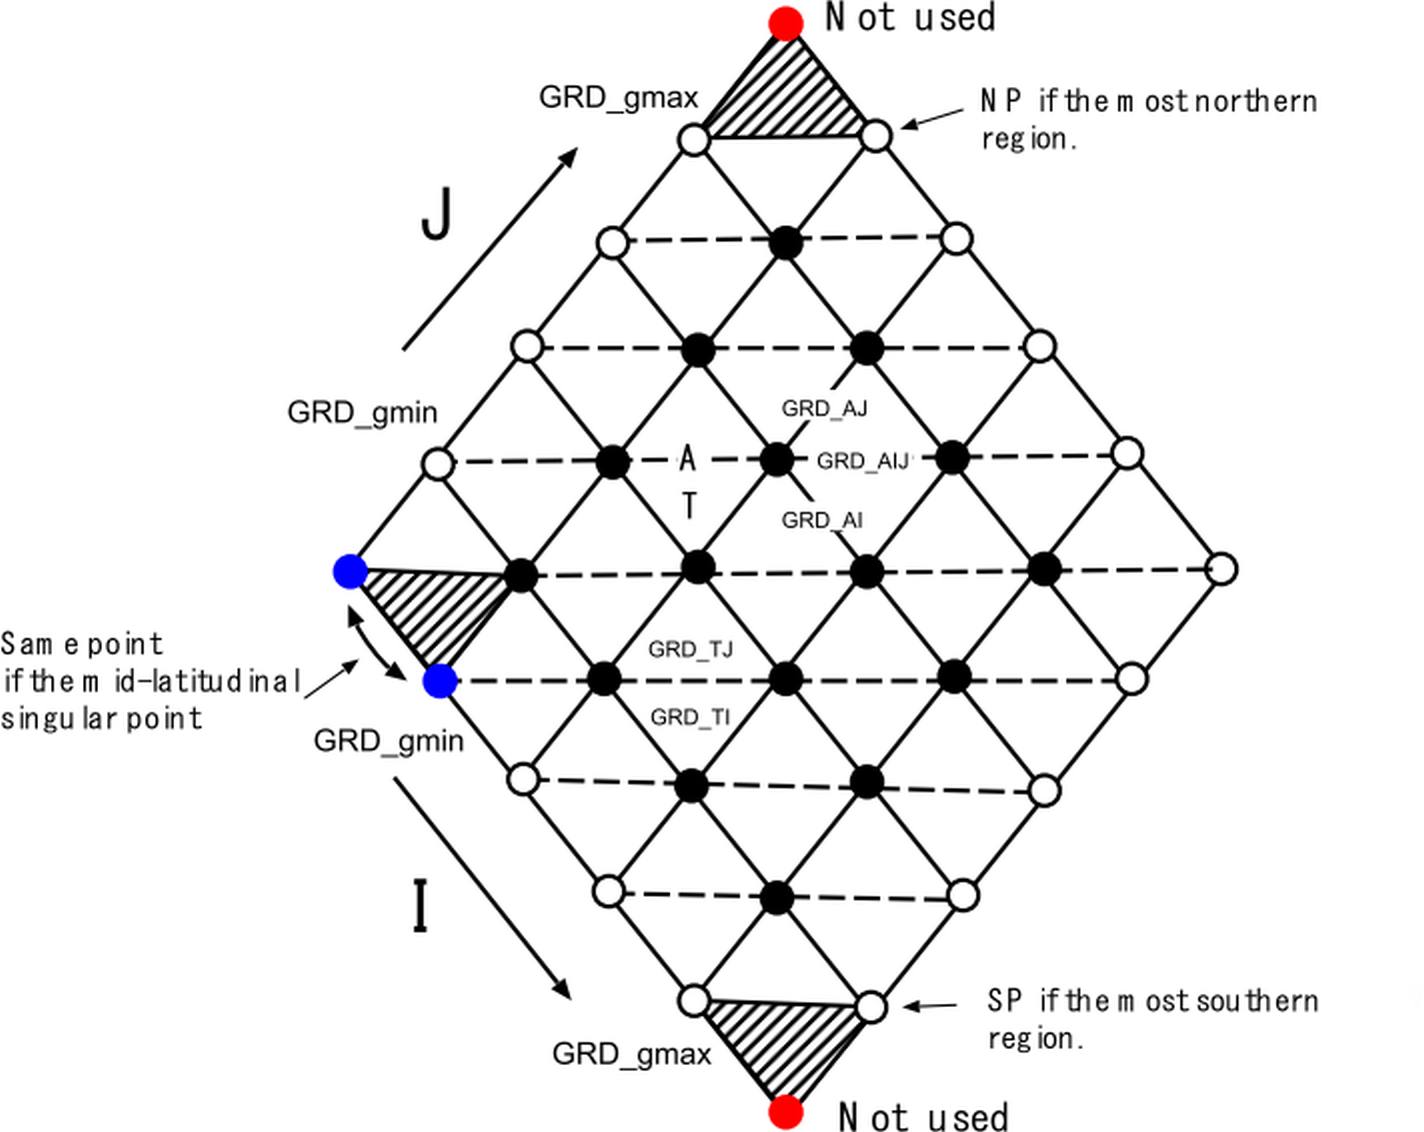
\includegraphics[scale=.5]{figs/Tomita2-12-0.png}
\caption{Schematic figure of data storing (regular region).}%
\label{f:data_store_regular}
\end{figure}



\begin{table}[htbp]
\centering
\caption{Data array for the regular region.}%
\label{t:data_array_regular}
\begin{tabular}{llll}
\hline\hline
 \multicolumn{4}{l}{\src{var(g,k,l)} : Grid point variables}\\
\hline
 $g$ & $=$ & $1 \ldots $ \text{\src{ADM_gall}} & horizontal index \\
 $k$ & $=$ & $1 \ldots $ \text{\src{ADM_kall}} & vertical index \\
 $l$ & $=$ & $1 \ldots $ \text{\src{ADM_lall}} & region index \\
\hline
 \multicolumn{4}{l}{\src{var(g,k,l,m)} : Triangle point variables}\\
\hline
 $g$ & $=$ & $1 \ldots $ \text{\src{ADM_gall}} & horizontal index \\
 $k$ & $=$ & $1 \ldots $ \text{\src{ADM_kall}} & vertical index \\
 $l$ & $=$ & $1 \ldots $ \text{\src{ADM_lall}} & region index \\
 $m$ & $=$ & \src{ADM_TI, ADM_TJ} & index of triangle position \\
\hline
 \multicolumn{4}{l}{\src{var(g,k,l,m)} : Arc point variables}\\
\hline
 $g$ & $=$ & $1 \ldots $ \text{\src{ADM_gall}} & first horizontal index \\
 $k$ & $=$ & $1 \ldots $ \text{\src{ADM_kall}} & vertical index \\
 $l$ & $=$ & $1 \ldots $ \text{\src{ADM_lall}} & region index \\
 $m$ & $=$ & \src{ADM_AI, ADM_AIJ, ADM_AJ} & index of arc position \\
\hline\hline
\end{tabular}
\end{table}


\subsection{Data array for pole region}

For pole region, \autoref{f:data_store_pole} shows the schematic figure
of data storing.
%
Only one grid point, the pole point, is managed, and the other point
marked by the white circles are the halo points, these are used only for
the reference and their values are provided from the neighboring regions
by the MPI communication or memory copy.
%
The indices for these halo are in order of clockwise direction.
%
The first dimension is horizontal suffix, and the size \src{ADM_GALL_PL} is set to 6,
one for pole point and five for halo points.
%
The second dimension is vertical suffix, which is the same with the
regular region.
%
The third dimension is region, suffix, and the range is 1 to
\src{ADM_LALL_PL}, which is the number of pole regions, and set to 2
(North pole and South pole).

Different from the regular region, the number of triangle points and arc
points are the same with the halo points, these are no need for more
dimension, and stored as the same dimensions with the grid points.
But the range of index are from \src{ADM_GMIN_PL}(=2) to \src{ADM_GMAX_PL}(=6).




\begin{figure}[htbp]
 \centering
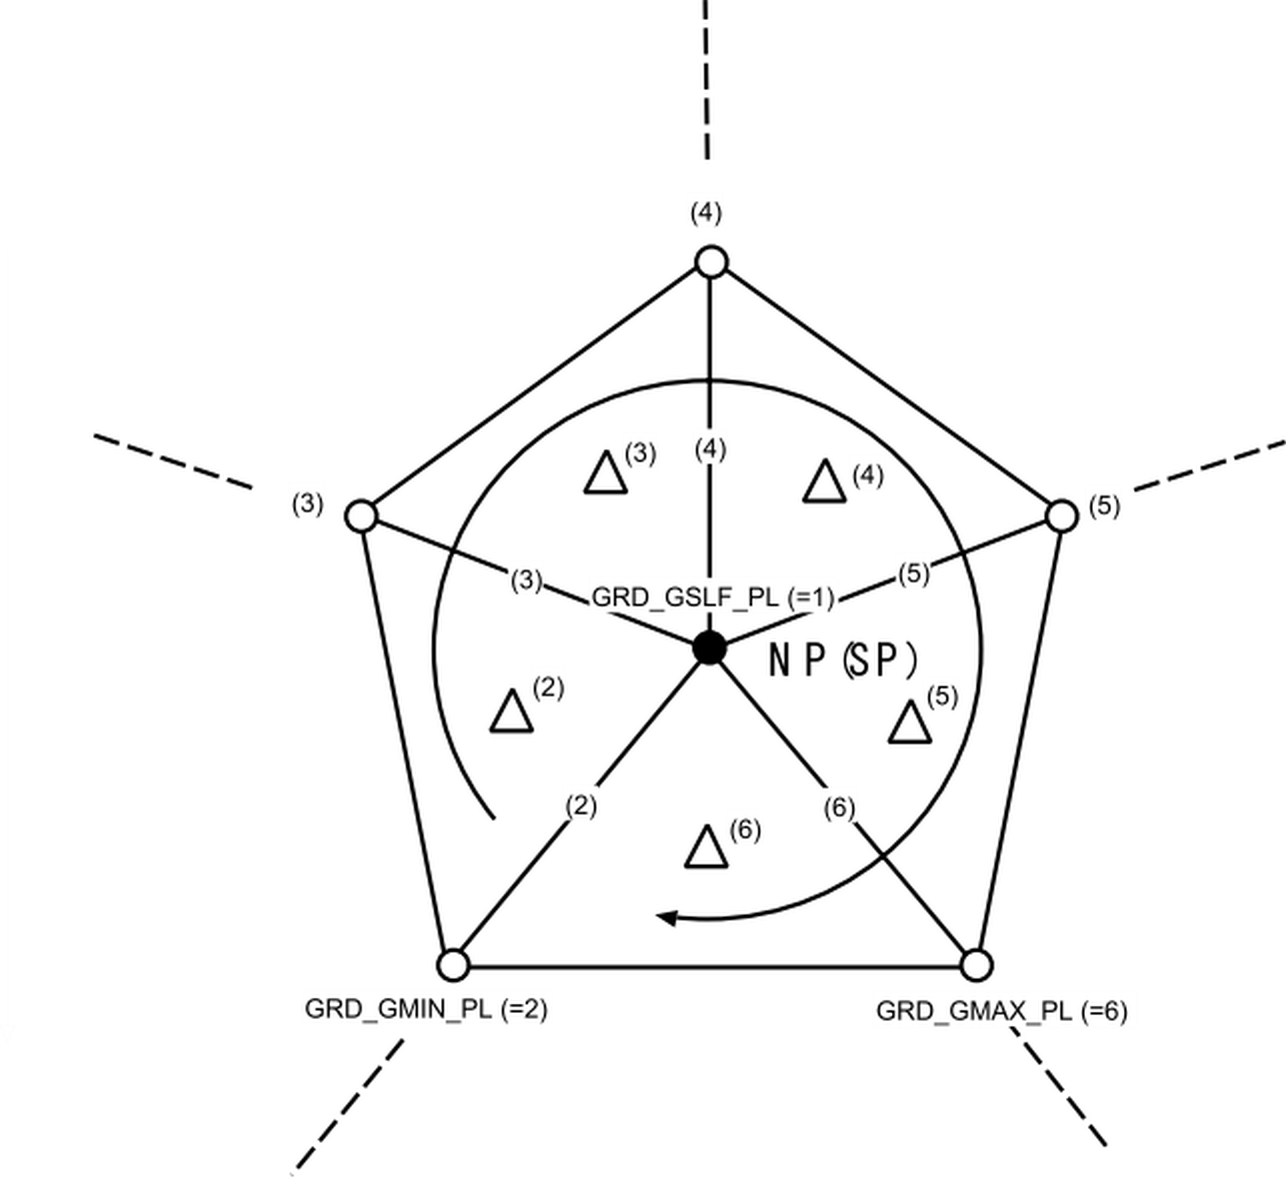
\includegraphics[scale=.5]{figs/Tomita2-12-1.png}
\caption{Schematic figure of data storing (pole region).}
\label{f:data_store_pole}
\end{figure}


\begin{table}[htbp]
\centering
\caption{Data array for the pole region.}
\begin{tabular}{llll}
\hline\hline
 \multicolumn{4}{l}{\src{var_pl(n,k,l)} : Grid, triangle, arc point variables}\\
\hline
 $n$ & $=$ & $1 \ldots $ \text{\src{ADM_GALL_PL}} & horizontal index \\
 $k$ & $=$ & $1 \ldots $ \text{\src{ADM_kall}} & vertical index \\
 $l$ & $=$ & $1 \ldots $ \text{\src{ADM_LALL_PL}} & region index \\
\hline
\end{tabular}
\end{table}

\subsection{Kernelize}

The kernels are single or multiple subroutines in original \NICAM source code,
and extracted and imposed into the wrapper for the kernel program.
%
Values of input variables in the argument list of the kernel subroutine
are stored as a data file just before the call in execution of the original \NICAM, and
they are read and given to the kernel subroutine in the kernel program.
%
Similarly values of output variables in the argument list are stored
just after the call in execution, and they are read and compared to the
actual output values of kernel subroutine, the difference are written to
the standard output for validation.

\NICAM uses several ``public object'' defined in several modules,
briefly described later.
%
Some of them are moved to \file{problem_size.inc} and \src{include}ed in
the \src{mod_misc}.



Kernel programs output several messages to the standard output, such as:
\begin{itemize}
%\setlength{\itemsep}{0pt}
 \item min/max/sum of input data,
 \item min/max/sum of output data,
 \item min/max/sum of difference between output and validation data,
 \item computational time (elapsed time).
\end{itemize}
%
Elapsed time is measured using \src{omp_get_wtime()}.

There are sample output file for the reference in \src{reference/} directory
of each kernel program, and also they are shown in``Input data and
result'' section of each kernel program in this document.

\subsection{Problem size}

In this kernel program package, problem size are set in
\file{problem_size.inc} in each kernel program, except
\src{communication}, as follows.
%
Number of grid point of one side of the region \src{ADM_gall_1d} is
$130$ including two halo points, and the total number of grid points in
whole region \src{ADM_gall} is $16900$, which corresponds to
$\text{glevel}-\text{rlevel}=7$.
%
Number of vertical layers \src{ADM_vlayer} is $40$ and the actual size
of $k$-direction \src{ADM_kall} is $42$.
%
The kernel program runs on a single process and this process manages
only one normal region, ie. \src{ADM_lall} is $1$, and also have two
pole regions, ie. \src{ADM_have_pl} is \src{.true.} and
\src{ADM_lall_pl} is $2$.
%
This normal region is to manage singular point, then
\src{ADM_have_sgp(1)} is \src{.true.}


\subsection{MPI and OpenMP}\label{s:mpi_openmpi}

While original \NICAM is parallelized by MPI and OpenMP,
all kernel program in this package except \src{communication}
are meant to be executed as one process and no threading.
%
And you don't need MPI library to compile/execute these kernel programs,
but you need to make OpneMP enable in order to use \src{omp_get_wtime()}.

\subsection{Mesuring environment}\label{s:measuring_env}

In the following sections, the example of performance result part of the
log output file of each kernel program is shown.
%
These were measured on the machine environment shown in
\autoref{t:machine_env},
with setting \src{export IAB_SYS=Ubuntu-gnu-ompi} on compilation 
(See \file{QuickStart.md}).


\begin{table}[htbp]
\centering
\caption{Measuring environment}\label{t:machine_env}
\small
\begin{tabularx}{.8\textwidth}{llX}
\hline
component & specification & notes \\ 
\hline
 CPU & Xeon E5-2630v4 @2.2GHz (10cores) x2 & HT disabled, TB enabled\\
 Memory & 256GB &\\
 Storage & SSD (SATA) &\\
 OS & Ubuntu 16.04.4 LTS &\\
 Compiler & GNU 5.4.0 & \\
 MPI & OpenMPI 1.10.2 & Ubuntu standard \\
\hline
\end{tabularx} 
\end{table}



